\documentclass{article}

% basics
\usepackage[utf8]{inputenc}
\usepackage[T1]{fontenc}
\usepackage{textcomp}
\usepackage{url}
\usepackage{hyperref}
\hypersetup{
    colorlinks,
    linkcolor={bb_g},
    citecolor={bb_g},
    urlcolor={bb_g}
}
\usepackage{graphicx}
\usepackage{float}
\usepackage{booktabs}
\usepackage{enumitem}
% \usepackage{parskip}
\usepackage{emptypage}
\usepackage{subcaption}
\usepackage{adjustbox}
\usepackage{multicol}
\usepackage[usenames,dvipsnames]{xcolor}

% \usepackage{cmbright}

\usepackage{amsmath, amsfonts, mathtools, amsthm, amssymb}
\usepackage[left=1.5in,right=1.5in,top=1.5in,bottom=1.5in]{geometry}
\usepackage{mathrsfs}
\usepackage{cancel}
\usepackage{bm}
\newcommand\N{\ensuremath{\mathbb{N}}}
\newcommand\R{\ensuremath{\mathbb{R}}}
\newcommand\Z{\ensuremath{\mathbb{Z}}}
\renewcommand\O{\ensuremath{\emptyset}}
\newcommand\Q{\ensuremath{\mathbb{Q}}}
\newcommand\C{\ensuremath{\mathbb{C}}}
\renewcommand{\qedsymbol}{$\blacksquare$}
\DeclareMathOperator{\sgn}{sgn}
\usepackage{systeme}
\let\svlim\lim\def\lim{\svlim\limits}
\let\implies\Rightarrow
\let\impliedby\Leftarrow
\let\iff\Leftrightarrow
\let\epsilon\varepsilon
\usepackage{stmaryrd} % for \lightning
\newcommand\contra{\scalebox{1.1}{$\lightning$}}
\let\phi\varphi
\newcommand{\petersengraph}{
	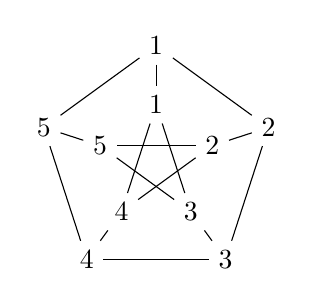
\begin{tikzpicture}[]
		\graph[clockwise, radius=1.5cm] {subgraph C_n [n=5,name=A] };
		\graph[clockwise, radius=.75cm] {subgraph I_n [n=5,name=B] };
	  
		\foreach \i [evaluate={\j=int(mod(\i+2+4,5)+1)}]% using Paul Gaborit's optimisation
		   in {1,2,3,4,5}{
		  \draw (A \i) -- (B \i);
		  \draw (B \j) -- (B \i);
		}
	\end{tikzpicture}
	}

% correct
\definecolor{correct}{HTML}{009900}
\newcommand\correct[2]{\ensuremath{\:}{\color{red}{#1}}\ensuremath{\to }{\color{correct}{#2}}\ensuremath{\:}}
\newcommand\green[1]{{\color{correct}{#1}}}


% Nord colors
\definecolor{d_0}{HTML}{2E3440}
\definecolor{d_1}{HTML}{3B4252}
\definecolor{d_2}{HTML}{434C5E}
\definecolor{d_3}{HTML}{4C566A}

\definecolor{w_0}{HTML}{D8DEE9}
\definecolor{w_1}{HTML}{E5E9F0}
\definecolor{w_2}{HTML}{ECEFF4}

\definecolor{b_ggg}{HTML}{8FBCBB}
\definecolor{b_gg}{HTML}{88C0D0}
\definecolor{b_g}{HTML}{81A1C1}
\definecolor{bb_g}{HTML}{5E81AC}

\definecolor{a_red}{HTML}{BF616A}
\definecolor{a_orange}{HTML}{D08770}
\definecolor{a_yellow}{HTML}{EBCB8B}
\definecolor{a_green}{HTML}{A3BE8C}
\definecolor{a_purple}{HTML}{B48EAD}


% Font
% \renewcommand{\familydefault}{\sfdefault}


% horizontal rule
\newcommand\hr{
    \noindent\rule[0.5ex]{\linewidth}{0.5pt}
}


% hide parts
\newcommand\hide[1]{}


% si unitx
\usepackage{siunitx}
\sisetup{locale = FR}
% \renewcommand\vec[1]{\mathbf{#1}}
\newcommand\mat[1]{\mathbf{#1}}


% tikz
\usepackage{tikz}
\usetikzlibrary{intersections, angles, quotes, positioning}
\usetikzlibrary{arrows.meta}
\usepackage{pgfplots}
\pgfplotsset{compat=1.13}


\tikzset{
	force/.style={thick, {Circle[length=2pt]}-stealth, shorten <=-1pt}
}

% quiver style
\usepackage{tikz-cd}
% `calc` is necessary to draw curved arrows.
\usetikzlibrary{calc}
% `pathmorphing` is necessary to draw squiggly arrows.
\usetikzlibrary{decorations.pathmorphing}

% A TikZ style for curved arrows of a fixed height, due to AndréC.
\tikzset{curve/.style={settings={#1},to path={(\tikztostart)
					.. controls ($(\tikztostart)!\pv{pos}!(\tikztotarget)!\pv{height}!270:(\tikztotarget)$)
					and ($(\tikztostart)!1-\pv{pos}!(\tikztotarget)!\pv{height}!270:(\tikztotarget)$)
					.. (\tikztotarget)\tikztonodes}},
	settings/.code={\tikzset{quiver/.cd,#1}
			\def\pv##1{\pgfkeysvalueof{/tikz/quiver/##1}}},
	quiver/.cd,pos/.initial=0.35,height/.initial=0}

% TikZ arrowhead/tail styles.
\tikzset{tail reversed/.code={\pgfsetarrowsstart{tikzcd to}}}
\tikzset{2tail/.code={\pgfsetarrowsstart{Implies[reversed]}}}
\tikzset{2tail reversed/.code={\pgfsetarrowsstart{Implies}}}
% TikZ arrow styles.
\tikzset{no body/.style={/tikz/dash pattern=on 0 off 1mm}}


% theorems
\makeatother
\usepackage{thmtools}
\usepackage[framemethod=TikZ]{mdframed}
\mdfsetup{skipabove=1em,skipbelow=0em}


\theoremstyle{definition}

\newcommand{\declaretheoremstylebox}[2]{
    \declaretheoremstyle[
        headfont=\bfseries\sffamily\color{#1}, bodyfont=\normalfont,
        mdframed={
            linewidth=2pt,
            rightline=false, topline=false, bottomline=false,
            linecolor=#1, backgroundcolor=#1!5
        }
    ]{thm#2box}    
}

\newcommand{\declaretheoremstyleline}[2]{
    \declaretheoremstyle[
        headfont=\bfseries\sffamily\color{#1}, bodyfont=\normalfont,
        mdframed={
            linewidth=2pt,
            rightline=false, topline=false, bottomline=false,
            linecolor=#1
        }
    ]{thm#2line}    
}

\declaretheoremstylebox{b_ggg}{green}
\declaretheoremstylebox{b_g}{blue}
\declaretheoremstylebox{a_red}{red}
\declaretheoremstylebox{a_orange}{orange}
\declaretheoremstylebox{a_yellow!60!a_orange}{yellow}

\declaretheoremstyleline{bb_g}{blue}
\declaretheoremstyleline{b_gg}{green}

\declaretheoremstyleline{d_3}{gray}

\declaretheoremstyle[
    headfont=\bfseries\sffamily\color{a_red}, bodyfont=\normalfont,
    numbered=no,
    mdframed={
        linewidth=2pt,
        rightline=false, topline=false, bottomline=false,
        linecolor=a_red, backgroundcolor=a_red!1,
    },
    qed=\qedsymbol
]{thmproofbox}

\declaretheoremstyle[
    headfont=\bfseries\sffamily\color{b_g}, bodyfont=\normalfont,
    numbered=no,
    mdframed={
        linewidth=2pt,
        rightline=false, topline=false, bottomline=false,
        linecolor=b_g, backgroundcolor=b_g!1,
    },
]{thmexplanationbox}

% \declaretheoremstyle[headfont=\bfseries\sffamily, bodyfont=\normalfont, mdframed={ nobreak } ]{thmgreenbox}
% \declaretheoremstyle[headfont=\bfseries\sffamily, bodyfont=\normalfont, mdframed={ nobreak } ]{thmredbox}
% \declaretheoremstyle[headfont=\bfseries\sffamily, bodyfont=\normalfont]{thmbluebox}
% \declaretheoremstyle[headfont=\bfseries\sffamily, bodyfont=\normalfont]{thmblueline}
% \declaretheoremstyle[headfont=\bfseries\sffamily, bodyfont=\normalfont, numbered=no, mdframed={ rightline=false, topline=false, bottomline=false, }, qed=\qedsymbol ]{thmproofbox}
% \declaretheoremstyle[headfont=\bfseries\sffamily, bodyfont=\normalfont, numbered=no, mdframed={ nobreak, rightline=false, topline=false, bottomline=false } ]{thmexplanationbox}

\declaretheorem[style=thmgreenbox, name=Definition]{definition}
\declaretheorem[style=thmbluebox, numbered=no, name=Example]{example}
\declaretheorem[style=thmorangebox, name=Proposition]{proposition}
\declaretheorem[style=thmredbox, name=Theorem]{theorem}
\declaretheorem[style=thmyellowbox, name=Lemma]{lemma}
\declaretheorem[style=thmredbox, numbered=no, name=Corollary]{corollary}

\declaretheorem[style=thmproofbox, name=Proof]{replacementproof}
\renewenvironment{proof}[1][\proofname]{\vspace{-10pt}\begin{replacementproof}}{\end{replacementproof}}

\declaretheorem[style=thmexplanationbox, name=Proof]{tmpexplanation}
\newenvironment{explanation}[1][]{\vspace{-10pt}\begin{tmpexplanation}}{\end{tmpexplanation}}

\declaretheorem[style=thmgreenline, numbered=no, name=Remark]{remark}
\declaretheorem[style=thmblueline, numbered=no, name=Note]{note}

\declaretheorem[style=thmgrayline, numbered=no, name=Question]{question}

\newtheorem*{uovt}{UOVT}
\newtheorem*{notation}{Notation}
\newtheorem*{previouslyseen}{As previously seen}
\newtheorem*{problem}{Problem}
\newtheorem*{observe}{Observe}
\newtheorem*{property}{Property}
\newtheorem*{intuition}{Intuition}


\usepackage{etoolbox}
\AtEndEnvironment{vb}{\null\hfill$\diamond$}%
\AtEndEnvironment{intermezzo}{\null\hfill$\diamond$}%
% \AtEndEnvironment{opmerking}{\null\hfill$\diamond$}%

% http://tex.stackexchange.com/questions/22119/how-can-i-change-the-spacing-before-theorems-with-amsthm
\makeatletter
% \def\thm@space@setup{%
%   \thm@preskip=\parskip \thm@postskip=0pt
% }


\newcommand{\exercise}[1]{%
    \def\@exercise{#1}%
    \subsection{Exercise #1}
}

\newcommand{\subexercise}[1]{%
    \subsubsection*{Exercise \@exercise.#1}
}


\usepackage{xifthen}

% Notes
\usepackage{marginnote}
\let\marginpar\marginnote

\def\testdateparts#1{\dateparts#1\relax}
\def\dateparts#1 #2 #3 #4 #5\relax{
    \marginpar{\small\textsf{\mbox{#1 #2 #3 #5}}}
}

\def\@lecture{}%
\newcommand{\lecture}[3]{
	\ifthenelse{\isempty{#3}}{%
		\def\@lecture{Lecture #1}%
	}{%
		\def\@lecture{Lecture #1: #3}%
	}%
	\section*{\@lecture}
	\marginpar{\small\textsf{\mbox{#2}}}
}


% \renewcommand\date[1]{\marginpar{#1}}


% fancy headers
\usepackage{fancyhdr}
\pagestyle{fancy}

% LE: left even
% RO: right odd
% CE, CO: center even, center odd
\fancyhead[LE, RO]{George C.}

\fancyhead[RO, LE]{\@lecture} % Right odd,  Left even
\fancyhead[RE, LO]{}          % Right even, Left odd
\fancyfoot[RO, LE]{\thepage}  % Right odd,  Left even
\fancyfoot[RE, LO]{}          % Right even, Left odd
\fancyfoot[C]{\leftmark}     % Center

\makeatother


% figure support
\usepackage{import}
\usepackage{xifthen}
\pdfminorversion=7
\usepackage{pdfpages}
\usepackage{transparent}
\newcommand{\incfig}[1]{%
    \def\svgwidth{\columnwidth}
    \import{./figures/}{#1.pdf_tex}
    }
    
%http://tex.stackexchange.com/questions/76273/multiple-pdfs-with-page-group-included-in-a-single-page-warning
\pdfsuppresswarningpagegroup=1

\setcounter{section}{-1}

\usetikzlibrary{graphs}
\usetikzlibrary{graphs.standard}

\title{Graph Theory}
\author{George C.}
\date{\today}

\pagecolor{d_0}

\begin{document}

\color{w_0}

\maketitle
\tableofcontents
\listoftheorems

\newpage

\lecture{1}{1/26/2023}{}

\section{Fundamental Concepts}
\begin{definition}[graph]
	\label{def:graph}
	A graph is a pair \((V,E)\) where \(V\) is the vertex space and \(E\) is the edge space.
\end{definition}

\begin{example}[petersen graph]
	\label{ex:petersen graph}
	An element subset of \(\{1,2,3,4,5\}\) connected by disjointedness
	\newcommand{\petersengraph}{
	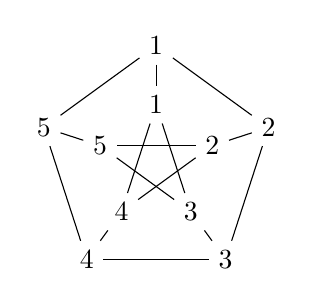
\begin{tikzpicture}[]
		\graph[clockwise, radius=1.5cm] {subgraph C_n [n=5,name=A] };
		\graph[clockwise, radius=.75cm] {subgraph I_n [n=5,name=B] };
	  
		\foreach \i [evaluate={\j=int(mod(\i+2+4,5)+1)}]% using Paul Gaborit's optimisation
		   in {1,2,3,4,5}{
		  \draw (A \i) -- (B \i);
		  \draw (B \j) -- (B \i);
		}
	\end{tikzpicture}
	}
	\[
		\petersengraph
	\]
\end{example}

\begin{note}
	In this course we are excluding multiple edges and self loops
\end{note}

\begin{definition}[vertex degrees]
	\label{def:vertex degrees}
	Let, \(G = (V, E)\), \(v \in V\), \(e \in E\)
	\(e\) are incident if \(v \in e\) i.e. \(v\) is an endpoint of \(e\)  
\end{definition}

\begin{lemma}
	\[
		\sum_{v \in V} deg(v) = \sum_{v \in V}\sum_{v \in e} 1 = \sum_{v \in e} \sum_{v \in V} 1 = 2 |E|  
	\]
\end{lemma}
\begin{proof}
	Every edge has two vertices
\end{proof}

\begin{definition}[complete graph]
	\label{def:complete graph}
	Represented \(K_n\), the graph has \(V = {1 \ldots n}\) and all possible edges
	\[
		|E| = \frac{n(n-1)}{2} = {n \choose 2}
	\]
\end{definition}

\begin{definition}[isomorphic]
	\label{def:isomorphic}
	Graphs \(G_1 = (V_1, E_1)\) and \(G_2 = (V_2, E_2)\) are isomorphic if there exists a bijection, \(f: v_1 \to v_2\), s.t. \(\{u, v\} \in E_1 \iff \{f(u), f(v)\} \in E_2\) 
\end{definition}

\subsection{Connectivity}
\begin{definition}[connected]
	\label{def:connected}
	\(u\) and \(v\) are connected if there exists a path from \(u\) to \(v\)
	A graph is connected when all vertices are connected   
\end{definition}


\lecture{2}{2023-01-31}{}

\subsection{Degree Sequences}
\begin{definition}[degree sequence]
	\label{def:degree sequence}
	List of vertex degrees in decreasing order
\end{definition}

\begin{note}
	Isomorphic graphs have the same degree sequence; however, if they have the same degree sequence they are not necessarily isomorphic
\end{note}

\begin{definition}[graphic]
	\label{def:graphic}
	A sequence is graphic if it's the \nameref{def:degree sequence} of some graph
\end{definition}

\begin{example} 
	Here are some degree sequences which may or may not exist:
	\begin{itemize}
		\item \((3,2,1,1)\) - not possible since they don't sum to an even number 
		\item \((3,3,1,1)\) - not graphic since there are not enough vertices
		\item \((3,2,2,1)\) - graphic
		% https://q.uiver.app/?q=WzAsNCxbMCwxLCJcXGJ1bGxldCJdLFsxLDAsIlxcYnVsbGV0Il0sWzEsMSwiXFxidWxsZXQiXSxbMSwyLCJcXGJ1bGxldCJdLFswLDEsIiIsMCx7InN0eWxlIjp7ImhlYWQiOnsibmFtZSI6Im5vbmUifX19XSxbMCwyLCIiLDIseyJzdHlsZSI6eyJoZWFkIjp7Im5hbWUiOiJub25lIn19fV0sWzAsMywiIiwyLHsic3R5bGUiOnsiaGVhZCI6eyJuYW1lIjoibm9uZSJ9fX1dLFsxLDIsIiIsMCx7InN0eWxlIjp7ImhlYWQiOnsibmFtZSI6Im5vbmUifX19XV0=
		\[\begin{tikzcd}
			& \bullet \\
			\bullet & \bullet \\
			& \bullet
			\arrow[no head, from=2-1, to=1-2]
			\arrow[no head, from=2-1, to=2-2]
			\arrow[no head, from=2-1, to=3-2]
			\arrow[no head, from=1-2, to=2-2]
		\end{tikzcd}\]
	\end{itemize}
\end{example} 

\begin{theorem}[Havel-Hakimi]
	\label{thm:havel-hakimi}
	\((a_1 \ldots a_n)\) is \nameref{def:graphic} iff \((a_{2}-1, a_{3}-1, \ldots a_{a_1+1}-1, \newline a_{a_1+2} \ldots a_n)\) is graphic
	
\end{theorem}
\begin{proof}
	We can apply the theorem in reverse to understand the intuition. If we have a graphic sequence, \((b_1 \ldots b_m )\), we can add a vertex with degree \(k\) such that  \((k , b_{1} +1, \ldots b_{k}+1, b_{k+1} \ldots b_m)\).
	% https://q.uiver.app/?q=WzAsNyxbMSwwLCJiXzEiXSxbMSwxLCJiXzMiXSxbMCwxLCJiXzIiXSxbMywwLCJrIl0sWzQsMCwiYl8xIl0sWzQsMSwiYl8zIl0sWzMsMSwiYl8yIl0sWzAsMSwiIiwwLHsic3R5bGUiOnsiaGVhZCI6eyJuYW1lIjoibm9uZSJ9fX1dLFsyLDAsIiIsMCx7InN0eWxlIjp7ImhlYWQiOnsibmFtZSI6Im5vbmUifX19XSxbMyw0LCIiLDAseyJzdHlsZSI6eyJoZWFkIjp7Im5hbWUiOiJub25lIn19fV0sWzMsNiwiIiwyLHsic3R5bGUiOnsiaGVhZCI6eyJuYW1lIjoibm9uZSJ9fX1dLFs2LDQsIiIsMix7InN0eWxlIjp7ImhlYWQiOnsibmFtZSI6Im5vbmUifX19XSxbNCw1LCIiLDIseyJzdHlsZSI6eyJoZWFkIjp7Im5hbWUiOiJub25lIn19fV0sWzcsMTAsIiIsMCx7InNob3J0ZW4iOnsic291cmNlIjoyMCwidGFyZ2V0IjoyMH19XV0=
	\[\begin{tikzcd}
		& {b_1} && k & {b_1} \\
		{b_2} & {b_3} && {b_2} & {b_3}
		\arrow[""{name=0, anchor=center, inner sep=0}, no head, 	from=1-2, to=2-2]
		\arrow[no head, from=2-1, to=1-2]
		\arrow[no head, from=1-4, to=1-5]
		\arrow[""{name=1, anchor=center, inner sep=0}, no head, 	from=1-4, to=2-4]
		\arrow[no head, from=2-4, to=1-5]
		\arrow[no head, from=1-5, to=2-5]
		\arrow[shorten <=13pt, shorten >=13pt, Rightarrow, 	from=0, to=1]
	\end{tikzcd}\]

	In the reverse direction, we can subtract a vertex from a graph, and we make a transformation (2-switch) which preserves degree sequences but makes the graph maximal, to get the reverse result.
\end{proof}

\begin{example}
	\((3,3,3,3,3,2,2,1)\) eventually becomes \((1,1,1,1,0)\) which we can show is graphic: 
	% https://q.uiver.app/?q=WzAsNSxbMywwLCJcXGJ1bGxldCJdLFswLDAsIlxcYnVsbGV0Il0sWzIsMCwiXFxidWxsZXQiXSxbMCwxLCJcXGJ1bGxldCJdLFsyLDEsIlxcYnVsbGV0Il0sWzEsMiwiIiwwLHsic3R5bGUiOnsiaGVhZCI6eyJuYW1lIjoibm9uZSJ9fX1dLFszLDQsIiIsMCx7InN0eWxlIjp7ImhlYWQiOnsibmFtZSI6Im5vbmUifX19XV0=
	\[\begin{tikzcd}
		\bullet && \bullet & \bullet \\
		\bullet && \bullet
		\arrow[no head, from=1-1, to=1-3]
		\arrow[no head, from=2-1, to=2-3]
	\end{tikzcd}\]
\end{example} 

\subsection{Bipartite graphs}
\begin{definition}[bipartitie graph]
	\label{def:bipartitie graph}
	A graph is bipartite if it's possible to color vertices using only 2 colors.
	A simple check for it being bipartite is to check if there are no odd cycles
\end{definition}

\subsection{Walks and Paths}
\begin{definition}[walk]
	\label{def:walk}
	A walk is a sequence of vertices that are connected by edges
	It has the property:
	\begin{definition}[length]
		\label{def:length}
		The number of edges contained in the walk
	\end{definition}
\end{definition}

\begin{definition}[path]
	\label{def:path}
	A path is a \nameref{def:walk} that has unique vertices
\end{definition}

\begin{lemma}
	A walk from \(v_{0}\) to \(v_n\) implies a path from \(v_{0}\) to \(v_n\) 
\end{lemma}

\subsection{Closed Walks and Cycles}
\begin{definition}[closed walk]
	\label{def:closed walk}
	A closed walk is a walk which starts and ends at the same vertex
\end{definition}
\begin{definition}[cycle]
	\label{def:cycle}
	A cycle is a \nameref{def:closed walk} that has unique vertices
\end{definition}

\begin{lemma}[closed walk]
	\label{lem:closedwalk}
	A closed walk of odd length contains an odd cycle
\end{lemma} 
\begin{proof}
	By induction:
	
	\emph{Base Case:} \(k=1\) A closed walk of length 3 (\(2k+1\) ) must be a cycle

	\emph{Inductive Step:} If all vertices in the walk are distinct we are done since it is a cycle of odd length. In the other case where there are repeated, we can split the walk on repeated vertices to get smaller walks which are proved in the previous cases
\end{proof}

\begin{theorem}[bipartie]
	\label{thm:bipartie}
	A graph is bipartite iff there are no odd cycles
\end{theorem} 

\lecture{3}{2023-02-02}{}

\begin{remark}
	Algorithmic Bipartite Testing
	\begin{itemize}
		\item Brute force: \(2^{| V |} \cdot | E |\) 
		\item Proof Algorithm: where we color the vertices and check the edges \(| V | + | E | \) 
	\end{itemize}
\end{remark}

\begin{remark}[local to global]
	\label{remark:local to global}
	Global properties always lead to local results (ex. bipartite implies no odd cycles). In West it is called "TONCAS"
\end{remark}

\subsection{Eulerian Graphs}

\begin{definition}[euler tour]
	\label{def:euler tour}
	A closed walk that visits each edge of a graph exactly once
\end{definition}

\begin{definition}[eulerian]
	\label{def:eulerian}
	A graph with an euler tour is Eulerian.
\end{definition}

\begin{proposition}[eulerian local property]
	\label{prop:eulerian local property}
	A graph is Eulerian iff every vertex has even degree.
\end{proposition}

\begin{example}[seven bridges of königsberg]
	\label{ex:seven bridges of königsberg}
	% https://q.uiver.app/?q=WzAsNCxbMCwxLCJcXGJ1bGxldCJdLFsyLDEsIlxcYnVsbGV0Il0sWzEsMCwiXFxidWxsZXQiXSxbMSwyLCJcXGJ1bGxldCJdLFswLDFdLFswLDIsIiIsMix7ImN1cnZlIjoxfV0sWzIsMV0sWzEsM10sWzMsMCwiIiwyLHsiY3VydmUiOi0xfV0sWzIsMCwiIiwyLHsiY3VydmUiOjF9XSxbMCwzLCIiLDIseyJjdXJ2ZSI6LTF9XV0=
\[\begin{tikzcd}
	& \bullet \\
	\bullet && \bullet \\
	& \bullet
	\arrow[from=2-1, to=2-3]
	\arrow[curve={height=6pt}, from=2-1, to=1-2]
	\arrow[from=1-2, to=2-3]
	\arrow[from=2-3, to=3-2]
	\arrow[curve={height=-6pt}, from=3-2, to=2-1]
	\arrow[curve={height=6pt}, from=1-2, to=2-1]
	\arrow[curve={height=-6pt}, from=2-1, to=3-2]
\end{tikzcd}\]
	Using a graph to model the seven bridges of Königsberg shows that an euler tour is not possible.
\end{example} 

\begin{note}
	This is another example of local and global properties where the parity of the degree is the local property and Eulerian is the global property
\end{note} 

\section{Trees}
\begin{definition}[tree]
	\label{def:tree}
	A tree is a \nameref{def:connected} and \hyperref[def:cycle]{acyclic} graph
\end{definition}

\begin{example}
	% https://q.uiver.app/?q=WzAsOSxbMCwxLCJcXGJ1bGxldCJdLFsxLDEsIlxcYnVsbGV0Il0sWzIsMCwiXFxidWxsZXQiXSxbMiwyLCJcXGJ1bGxldCJdLFszLDEsIlxcYnVsbGV0Il0sWzMsMiwiXFxidWxsZXQiXSxbNCwwLCJcXGJ1bGxldCJdLFs0LDEsIlxcYnVsbGV0Il0sWzUsMSwiXFxidWxsZXQiXSxbMCwxLCIiLDAseyJzdHlsZSI6eyJoZWFkIjp7Im5hbWUiOiJub25lIn19fV0sWzEsMiwiIiwwLHsic3R5bGUiOnsiaGVhZCI6eyJuYW1lIjoibm9uZSJ9fX1dLFsxLDMsIiIsMCx7InN0eWxlIjp7ImhlYWQiOnsibmFtZSI6Im5vbmUifX19XSxbMyw0LCIiLDAseyJzdHlsZSI6eyJoZWFkIjp7Im5hbWUiOiJub25lIn19fV0sWzMsNSwiIiwwLHsic3R5bGUiOnsiaGVhZCI6eyJuYW1lIjoibm9uZSJ9fX1dLFs0LDYsIiIsMCx7InN0eWxlIjp7ImhlYWQiOnsibmFtZSI6Im5vbmUifX19XSxbNCw3LCIiLDAseyJzdHlsZSI6eyJoZWFkIjp7Im5hbWUiOiJub25lIn19fV0sWzcsOCwiIiwwLHsic3R5bGUiOnsiaGVhZCI6eyJuYW1lIjoibm9uZSJ9fX1dXQ==
\[\begin{tikzcd}
	&& \bullet && \bullet \\
	\bullet & \bullet && \bullet & \bullet & \bullet \\
	&& \bullet & \bullet
	\arrow[no head, from=2-1, to=2-2]
	\arrow[no head, from=2-2, to=1-3]
	\arrow[no head, from=2-2, to=3-3]
	\arrow[no head, from=3-3, to=2-4]
	\arrow[no head, from=3-3, to=3-4]
	\arrow[no head, from=2-4, to=1-5]
	\arrow[no head, from=2-4, to=2-5]
	\arrow[no head, from=2-5, to=2-6]
\end{tikzcd}\]
\end{example}

\begin{definition}[leaf]
	\label{def:leaf}
	A node of degree \(1\) 
\end{definition}

\begin{lemma}
	Any connected subgraph of a tree is a tree 
\end{lemma}
\begin{proof}
	By contradiction:

	Assume that the connected subgraph is not a tree, then the subgraph has a cycle, therefore the graph has a cycle, but trees are acyclic. Therefore, contradiction.
\end{proof}

\begin{lemma}
	A tree with \(n\) vertices has \(n-1\) edges
\end{lemma}
\begin{proof}
	By induction:
	
	\emph{Base Case:} There are \(0\) edges in a \(1\) vertex tree

	\emph{Inductive Step:} Suppose this holds for \(n\).
	Let \(T\) be a tree with \(n+1\) vertices, then by removing one vertex, which must be a leaf — removing a non-leaf would make the graph unconnected, you remove one edge and the graph becomes the \(n\) case.
	Therefore, the \(n+1\) tree has \(1\) more edge than an \(n\) tree.
\end{proof}

\subsection{Spanning Trees}
\begin{definition}[spanning tree]
	\label{def:spanning tree}
	A spanning tree (ST) is a subgraph of a \nameref{def:connected} that is a \nameref{def:tree} that contains all vertices of the original graph
\end{definition}

\begin{lemma}
	There is a spanning tree in every connected graph
\end{lemma}
\begin{proof}
	By contradiction: \\
	Assume \(G\) is a connected graph with no ST.
	Let \(T\) be a connected subgraph of \(G\)  that has the same vertices as \(G\) with the smallest number of edges. Since \(T\) is not a tree, it does not have a cycle. However, \(T\) containing a cycle would imply that \(T\) is not a subgraph that has the smallest number of edges.
	Therefore, contradiction test 
\end{proof}

\begin{proposition}
    With a graph \(G\) where \(T, T^\prime \subset G\) s.t. \(e \in T, e \notin T^\prime\). Then there is edge \(e^\prime \in T^\prime \) s.t. \(T - e + e^\prime\)  is a spanning tree.
\end{proposition}
\begin{proof}
    \(T\) is a tree \(\implies\) \(T - e\) is disconnected. \(T, T^\prime\) have the same vertex set \(\implies \exists e \in T^\prime\) that connects two components of \(T - e\) Lets claim that \(T - e + e^\prime\) is a spanning tree. It has the same number of edges and is connected, so it's a tree, and is spanning since it connects all edges. 
\end{proof}

\lecture{4}{2023-02-09}{}

Prüfer Code to Tree 

\begin{example}[Prufer Code to Tree]
    \label{ex:prufer code to tree}
    Let's take the example \((1,4,1,1)\)

    We know that vertices of deg \(1\) do not appear, so we start with an edge from \(2\) to \(1\)  then we remove \(1\) from the list. Next we start with \(4\) and add the next deg \(1\) vertex. Now we have a connection from \(4\) to \(1\) since it's left in the Prüfer code. Then we finally create a tree with vertices \(1,5,6\) and adjoin it.
\end{example} 

\begin{theorem}[1]
    \label{thm:1}
    For each sequence \((\vec{a_1} \ldots a_{n-2})\) there exists a unique tree \(T\) with \(P(T) = (\vec{a_1} \ldots a_{n-2})\)
\end{theorem}
\begin{proof}
    By induction:
    
    \emph{Base Case:} \(n = 2\)
    sequences have length \(n = 2 = 0\) and there is only one tree with \(2\) vertices

    \emph{Inductive Step:}
    For any tree with code \((\vec{a_1} \ldots a_{n-2})\) Let \(x\) be the smallest index not in the sequence then we can construct an edge between it and \(a_1\) and remove \(a_1\) from the code. Therefore, we have a code with one less element. And, by induction, \(\exists !\) a tree \(T^\prime\) with vertices \(\{1\ldots n\}\setminus{x}\)  and code \((a_2 \ldots a_{n-2})\).

    The uniqueness come from the fact that \(T^\prime\) is unique and there is only one way to add an edge
\end{proof}
\begin{corollary}[cayley]
    \label{cor:cayley}
    There is a bijection between trees and these sequences. Therefore, we can count trees easily by counting sequences.
\end{corollary}



\lecture{5}{2023-02-14}{}

\section*{Matchings}

\begin{definition}[matching]
    \label{def:matching}
    A matching is a subset of \(M \subset E\) such that no two edges in \(M\) share a vertex  
\end{definition}

\begin{definition}[saturates]
    \label{def:saturates}
    For \(U \subset V\) say \(M\) saturates \(U\) if each \(u \in U\) is incident to some \(e \in M\) A matching that saturates \(V\) is called perfect
\end{definition}  

Perfect matching relate to bijections. 

\subsection*{Matchings in Bipartite Graphs}

For \(G = (X \sqcup Y, E)\), is there a matching that saturates \(X\)?
\begin{example}
    % https://q.uiver.app/?q=WzAsNixbMCwwLCJcXGJ1bGxldCJdLFswLDEsIlxcYnVsbGV0Il0sWzEsMSwiXFxidWxsZXQiXSxbMSwwLCJcXGJ1bGxldCJdLFsyLDEsIlxcYnVsbGV0Il0sWzIsMCwiXFxidWxsZXQiXSxbMCwxLCIiLDAseyJzdHlsZSI6eyJib2R5Ijp7Im5hbWUiOiJkb3R0ZWQifSwiaGVhZCI6eyJuYW1lIjoibm9uZSJ9fX1dLFswLDIsIiIsMix7InN0eWxlIjp7ImhlYWQiOnsibmFtZSI6Im5vbmUifX19XSxbMywyLCIiLDAseyJzdHlsZSI6eyJoZWFkIjp7Im5hbWUiOiJub25lIn19fV0sWzMsNCwiIiwyLHsic3R5bGUiOnsiYm9keSI6eyJuYW1lIjoiZG90dGVkIn0sImhlYWQiOnsibmFtZSI6Im5vbmUifX19XSxbNSw0LCIiLDAseyJzdHlsZSI6eyJoZWFkIjp7Im5hbWUiOiJub25lIn19fV0sWzUsMiwiIiwwLHsic3R5bGUiOnsiYm9keSI6eyJuYW1lIjoiZG90dGVkIn0sImhlYWQiOnsibmFtZSI6Im5vbmUifX19XSxbNSwxLCIiLDIseyJzdHlsZSI6eyJoZWFkIjp7Im5hbWUiOiJub25lIn19fV0sWzMsMSwiIiwxLHsic3R5bGUiOnsiaGVhZCI6eyJuYW1lIjoibm9uZSJ9fX1dLFswLDQsIiIsMSx7InN0eWxlIjp7ImhlYWQiOnsibmFtZSI6Im5vbmUifX19XV0=
\[\begin{tikzcd}
	\bullet & \bullet & \bullet \\
	\bullet & \bullet & \bullet
	\arrow[dotted, no head, from=1-1, to=2-1]
	\arrow[no head, from=1-1, to=2-2]
	\arrow[no head, from=1-2, to=2-2]
	\arrow[dotted, no head, from=1-2, to=2-3]
	\arrow[no head, from=1-3, to=2-3]
	\arrow[dotted, no head, from=1-3, to=2-2]
	\arrow[no head, from=1-3, to=2-1]
	\arrow[no head, from=1-2, to=2-1]
	\arrow[no head, from=1-1, to=2-3]
\end{tikzcd}\]
\end{example}

\begin{proposition}
    Local to Global: (Saturated Matching for Bipartite Graph)
    Let \(N(S)\) be set of vertices connected to vertices in \(S\). The local property is that for \(S \in X\), \(|S| \leq |N(S)|\)   
\end{proposition}

\begin{theorem}[Hall's Matching]
    \label{thm:hall's matching}
    \(G = (X \sqcup Y, E)\)  bipartite has matching saturating \(X\) iff \((\forall S \subset X)(|S| \leq |N(S)|)\)
\end{theorem}
\begin{proof}
	The proof requires \refname{maximum matching} theorem.
	Suppose \(G\) does not have a matching that saturates \(X\). 
	Let \(M\) max matching that does not saturate \(X\), \(u \in X\) unsaturated. \(S = \{x \in X \text{connected to u by a M-alt path} \}\)  \(T = \{y \in Y \text{connected to u by a M-alt path} \}\) Any M-alt path from \(u\) to \( y \in T\)  can be extended uniquesly to M-alt path ending in \(S\) Therefore, there is a bijection from \(T\) to \(S \setminus u\) \(N(S) = T\) since \(T \subset N(S)\) by definition and \(N(S) \subset T\) because we can fix a \(y \in N(S)\) which is connected to an \(x\)  which is connected to \(u\).
\end{proof} 
\begin{corollary}
    Any k-regular bipartite graph has perfect matching	
\end{corollary}
\begin{proof}
    Fix \(G = (X \cup Y, E)\) bipartite and k=regular

    Show \(|X| = |Y|\): \(k|X| = \sum_{x \in X} deg(x) = |E| = \sum_{y \in Y} deg(y) = k|Y|\)
    Fix \(S \in X\). Each edge leaving \(S\)  lands in \(N(S)\). There are \(k|N(S)|\) edges entering \(N|S|\). Therefore, \(k|S| \leq k|N(S)\).
    % https://q.uiver.app/?q=WzAsNixbMCwwLCJzIl0sWzIsMCwibiJdLFsyLDEsIm4iXSxbMiwyLCJuIl0sWzAsMSwicyJdLFswLDMsInYgXFxub3RpbiBTIl0sWzAsMV0sWzAsMl0sWzAsM10sWzQsMV0sWzQsMl0sWzQsM10sWzUsM10sWzUsMl0sWzUsMV1d
\[\begin{tikzcd}
	s && n \\
	s && n \\
	&& n \\
	{v \notin S}
	\arrow[from=1-1, to=1-3]
	\arrow[from=1-1, to=2-3]
	\arrow[from=1-1, to=3-3]
	\arrow[from=2-1, to=1-3]
	\arrow[from=2-1, to=2-3]
	\arrow[from=2-1, to=3-3]
	\arrow[from=4-1, to=3-3]
	\arrow[from=4-1, to=2-3]
	\arrow[from=4-1, to=1-3]
\end{tikzcd}\]
\end{proof}

\subsection*{Matching Duel Problem}
\begin{definition}[maximium]
    \label{def:maximium}
    A matching \(M \in E\) is maximum if it has the most edges of any matching
\end{definition}

Given \(G\) what is the size of it's maximum matching?

There exists an upper bound for this problem

\begin{definition}[vertex cover]
    \label{def:vertex cover}
    A vertex cover of \(G\)  is a subset \(Q \subset V\) s.t. every edge is incident to some vertex in \(Q\)
    % https://q.uiver.app/?q=WzAsMTMsWzIsMSwiXFxidWxsZXQiXSxbMywwLCJcXGJ1bGxldCJdLFs0LDAsIlxcYnVsbGV0Il0sWzUsMSwiXFxidWxsZXQiXSxbNCwyLCJcXGJ1bGxldCJdLFszLDIsIlxcYnVsbGV0Il0sWzIsMywiXFxidWxsZXQiXSxbMSwzLCJcXGJ1bGxldCJdLFswLDIsIlxcYnVsbGV0Il0sWzEsMSwiXFxidWxsZXQiXSxbMyw0LCJcXGJ1bGxldCJdLFs0LDQsIlxcYnVsbGV0Il0sWzUsMywiXFxidWxsZXQiXSxbMCwxLCIiLDAseyJzdHlsZSI6eyJoZWFkIjp7Im5hbWUiOiJub25lIn19fV0sWzEsMiwiIiwwLHsic3R5bGUiOnsiaGVhZCI6eyJuYW1lIjoibm9uZSJ9fX1dLFsyLDMsIiIsMCx7InN0eWxlIjp7ImhlYWQiOnsibmFtZSI6Im5vbmUifX19XSxbMyw0LCIiLDAseyJzdHlsZSI6eyJoZWFkIjp7Im5hbWUiOiJub25lIn19fV0sWzQsNSwiIiwwLHsic3R5bGUiOnsiaGVhZCI6eyJuYW1lIjoibm9uZSJ9fX1dLFs1LDAsIiIsMCx7InN0eWxlIjp7ImhlYWQiOnsibmFtZSI6Im5vbmUifX19XSxbNSw2LCIiLDAseyJzdHlsZSI6eyJoZWFkIjp7Im5hbWUiOiJub25lIn19fV0sWzYsNywiIiwwLHsic3R5bGUiOnsiaGVhZCI6eyJuYW1lIjoibm9uZSJ9fX1dLFs3LDgsIiIsMCx7InN0eWxlIjp7ImhlYWQiOnsibmFtZSI6Im5vbmUifX19XSxbOCw5LCIiLDAseyJzdHlsZSI6eyJoZWFkIjp7Im5hbWUiOiJub25lIn19fV0sWzksMCwiIiwwLHsic3R5bGUiOnsiaGVhZCI6eyJuYW1lIjoibm9uZSJ9fX1dLFs2LDEwLCIiLDAseyJzdHlsZSI6eyJoZWFkIjp7Im5hbWUiOiJub25lIn19fV0sWzEwLDExLCIiLDAseyJzdHlsZSI6eyJoZWFkIjp7Im5hbWUiOiJub25lIn19fV0sWzExLDEyLCIiLDAseyJzdHlsZSI6eyJoZWFkIjp7Im5hbWUiOiJub25lIn19fV0sWzEyLDQsIiIsMCx7InN0eWxlIjp7ImhlYWQiOnsibmFtZSI6Im5vbmUifX19XV0=
\[\begin{tikzcd}
	&&& \bullet & \bullet \\
	& \bullet & \bullet &&& \bullet \\
	\bullet &&& \bullet & \bullet \\
	& \bullet & \bullet &&& \bullet \\
	&&& \bullet & \bullet
	\arrow[no head, from=2-3, to=1-4]
	\arrow[no head, from=1-4, to=1-5]
	\arrow[no head, from=1-5, to=2-6]
	\arrow[no head, from=2-6, to=3-5]
	\arrow[no head, from=3-5, to=3-4]
	\arrow[no head, from=3-4, to=2-3]
	\arrow[no head, from=3-4, to=4-3]
	\arrow[no head, from=4-3, to=4-2]
	\arrow[no head, from=4-2, to=3-1]
	\arrow[no head, from=3-1, to=2-2]
	\arrow[no head, from=2-2, to=2-3]
	\arrow[no head, from=4-3, to=5-4]
	\arrow[no head, from=5-4, to=5-5]
	\arrow[no head, from=5-5, to=4-6]
	\arrow[no head, from=4-6, to=3-5]
\end{tikzcd}\]
\end{definition}

\begin{lemma}
    Let \(Q \subseteq V\) be a vertex cover of \(G\), then matching of \(G\) has at most \(Q\) edges
\end{lemma}

\begin{remark}
    Matchings and vertex covers are dual problems
\end{remark}

\lecture{6}{2023-02-16}{}

\begin{lemma}
	Let \(Q\) be a vertex cover, \(M\) a matching
	Then \(|M| \leq |Q|\) 
\end{lemma}
\begin{proof}
	For each \(e \in M\) there is at least one vertex of \(Q\) incident to \(e\). No two \(e, e^\prime \in M\) share a vertex of \(Q\)
\end{proof}

We can use this to show that if we have a vertex cover that covers all vertices with the same number of a matching we have a maximum matching.

\begin{theorem}[König]
	\label{thm:könig}
	Let \(G\) bipartite, then the max size of the matching is equal to the min size of the vertex cover
\end{theorem} 

Therefore, matching and vertex covers are duel problems

\begin{definition}[M-augmenting-path]
	\label{def:m-augmenting-path}
	A path whose edges alternate between \(M\) and \(E\setminus M\) whose end points are unsaturated.

	% picture spquare and hexagon
\end{definition}  

Local property for max matchings: If there exists an M-agumenting path then M is not maximum

\begin{theorem}[maximum matching]
	\label{thm:maximum matching}
	If there's no M-augmenting path then \(M\)  is maximium
\end{theorem}
\begin{proof}
	\begin{note}
		Suppose \(M\) is not a maximium there exists a \(M^\prime\) s.t. \(|m| < | M^\prime|\) consider the symmetric diffrence \(M \triangle M^\prime\). Here vertices have either degree \(1\) or \(2\) and the graph is aunion of even cycles and paths. 
	\end{note}
	Let \(M\) be a non maximal matching, \(M^\prime\) maximum matching. Consider \(M \triangle M^\prime\) By above this is a union of paths and even cycles. Since \(M\) and \(M^\prime\) share the same size in cycles then some compoent in \(M \triangle M^\prime\) has a path
\end{proof}




\lecture{7}{2023-02-23}{}

\begin{definition}[matching — stable]
    \label{def:matching — stable}
    A matching is stable if 
    % https://q.uiver.app/?q=WzAsNCxbMCwwLCJ4Il0sWzEsMSwieVxccHJpbWUiXSxbMSwwLCJ4XFxwcmltZSJdLFswLDEsInkiXSxbMCwzLCIiLDAseyJzdHlsZSI6eyJoZWFkIjp7Im5hbWUiOiJub25lIn19fV0sWzIsMSwiIiwyLHsic3R5bGUiOnsiaGVhZCI6eyJuYW1lIjoibm9uZSJ9fX1dLFswLDEsIiIsMCx7InN0eWxlIjp7ImJvZHkiOnsibmFtZSI6ImRvdHRlZCJ9LCJoZWFkIjp7Im5hbWUiOiJub25lIn19fV1d
\[\begin{tikzcd}
	x & x\prime \\
	y & y\prime
	\arrow[no head, from=1-1, to=2-1]
	\arrow[no head, from=1-2, to=2-2]
	\arrow[dotted, no head, from=1-1, to=2-2]
\end{tikzcd}\]
    then either \(x\) prefers \(y\) to \(y^\prime\) or \(y^\prime\) prefers \(x^\prime\) to x
\end{definition}  

\begin{theorem}[Gale-Shapely]
    \label{thm:gale-shapely}
    Stable matchings always exist in bipartite graphs
\end{theorem} 
\begin{proof}
    We preform an algorithm to construct a stable matching:
    \begin{enumerate}
        \item[Round 1] 
        Each \(x \in X\) proposes to top choice
        
        Each \(y \in Y\) accepts the highest proposal
        \item[Subsequent rounds] Each unmatched \(x\) proposes to top choice not yet proposed to. Each \(y\) accepts the best proposal possible breaking an engagement

        \item[Repeat]
    \end{enumerate}
    
    \emph{Features}
    \begin{enumerate}
        \item Algorithm stops after \(<|E|\) rounds
        \item End matching is stable
        \item Proposers get the best match among all stable matchings. Proposees get worse 
    \end{enumerate}
\end{proof}

\begin{example}
    % https://q.uiver.app/?q=WzAsMTIsWzAsMCwiYSJdLFswLDEsImQiXSxbMSwxLCJlIl0sWzEsMCwiYiJdLFsyLDEsImYiXSxbMiwwLCJjIl0sWzMsMCwiXFxidWxsZXQiXSxbMywxLCJcXGJ1bGxldCJdLFs0LDEsIlxcYnVsbGV0Il0sWzQsMCwiXFxidWxsZXQiXSxbNSwxLCJcXGJ1bGxldCJdLFs1LDAsIlxcYnVsbGV0Il0sWzEsMCwiMywxIiwzLHsic3R5bGUiOnsiaGVhZCI6eyJuYW1lIjoibm9uZSJ9fX1dLFswLDIsIiIsMix7InN0eWxlIjp7ImhlYWQiOnsibmFtZSI6Im5vbmUifX19XSxbMyw0LCIiLDIseyJzdHlsZSI6eyJoZWFkIjp7Im5hbWUiOiJub25lIn19fV0sWzAsNCwiIiwyLHsic3R5bGUiOnsiaGVhZCI6eyJuYW1lIjoibm9uZSJ9fX1dLFszLDEsIiIsMSx7InN0eWxlIjp7ImhlYWQiOnsibmFtZSI6Im5vbmUifX19XSxbMywyLCIiLDEseyJzdHlsZSI6eyJoZWFkIjp7Im5hbWUiOiJub25lIn19fV0sWzUsMSwiIiwxLHsic3R5bGUiOnsiaGVhZCI6eyJuYW1lIjoibm9uZSJ9fX1dLFs1LDIsIiIsMSx7InN0eWxlIjp7ImhlYWQiOnsibmFtZSI6Im5vbmUifX19XSxbNSw0LCIiLDEseyJzdHlsZSI6eyJoZWFkIjp7Im5hbWUiOiJub25lIn19fV0sWzYsNywiIiwxLHsic3R5bGUiOnsiaGVhZCI6eyJuYW1lIjoibm9uZSJ9fX1dLFs2LDgsIiIsMSx7InN0eWxlIjp7ImJvZHkiOnsibmFtZSI6InNxdWlnZ2x5In0sImhlYWQiOnsibmFtZSI6Im5vbmUifX19XSxbOSw3LCIiLDEseyJzdHlsZSI6eyJoZWFkIjp7Im5hbWUiOiJub25lIn19fV0sWzksOCwiIiwxLHsic3R5bGUiOnsiaGVhZCI6eyJuYW1lIjoibm9uZSJ9fX1dLFs5LDEwLCIiLDEseyJzdHlsZSI6eyJib2R5Ijp7Im5hbWUiOiJzcXVpZ2dseSJ9LCJoZWFkIjp7Im5hbWUiOiJub25lIn19fV0sWzExLDgsIiIsMSx7InN0eWxlIjp7ImhlYWQiOnsibmFtZSI6Im5vbmUifX19XSxbMTEsMTAsIiIsMSx7InN0eWxlIjp7ImhlYWQiOnsibmFtZSI6Im5vbmUifX19XSxbMTEsNywiIiwxLHsic3R5bGUiOnsiYm9keSI6eyJuYW1lIjoic3F1aWdnbHkifSwiaGVhZCI6eyJuYW1lIjoibm9uZSJ9fX1dLFs2LDEwLCIiLDEseyJzdHlsZSI6eyJoZWFkIjp7Im5hbWUiOiJub25lIn19fV1d
\[\begin{tikzcd}
	a & b & c & \bullet & \bullet & \bullet \\
	d & e & f & \bullet & \bullet & \bullet
	\arrow["{3,1}"{marking}, no head, from=2-1, to=1-1]
	\arrow[no head, from=1-1, to=2-2]
	\arrow[no head, from=1-2, to=2-3]
	\arrow[no head, from=1-1, to=2-3]
	\arrow[no head, from=1-2, to=2-1]
	\arrow[no head, from=1-2, to=2-2]
	\arrow[no head, from=1-3, to=2-1]
	\arrow[no head, from=1-3, to=2-2]
	\arrow[no head, from=1-3, to=2-3]
	\arrow[no head, from=1-4, to=2-4]
	\arrow[squiggly, no head, from=1-4, to=2-5]
	\arrow[no head, from=1-5, to=2-4]
	\arrow[no head, from=1-5, to=2-5]
	\arrow[squiggly, no head, from=1-5, to=2-6]
	\arrow[no head, from=1-6, to=2-5]
	\arrow[no head, from=1-6, to=2-6]
	\arrow[squiggly, no head, from=1-6, to=2-4]
	\arrow[no head, from=1-4, to=2-6]
\end{tikzcd}\]
\end{example}
\lecture{8}{2023-02-28}{}

\section{Connectivity}

\begin{definition}[vertex cut]
	\label{def:vertex cut}
	A vertex cut on a graph \(G\) is a subset \(S \subset V\) s.t. \(G \setminus S\) is disconnected
\end{definition}  

\begin{definition}[vertex connectivity]
	\label{def:vertex connectivity}
	The vertex connectivity, \(\kappa (G)\) , is the min of the vertex cut
	\(\kappa (K_n)\) is not defined 
\end{definition}

\begin{lemma}
	If \(G\) is not complete then \(G\)  has a vertex cut
\end{lemma} 
\begin{proof}
	Let \(G\) not be complete, then there exist \(u, v \in V\)  s.t. \(\{u,v\} \notin E\). Then \(S = V\setminus{u, v}\) is a vertex cut
\end{proof}

\subsection{Connectivity Duel Problem}
Let \(G = (V,E)\). for \(x, y \in V\) define \(\kappa (x,y)\) min size of vertex cut that disconnects \(x\) and \(y\)

\begin{note}
	We see that the points we have to remove are related to paths from \(x\) to \(y\) which have no intersection.
\end{note} 

\begin{definition}[disjoint path]
	\label{def:disjoint path}
	A path is disjoint with another path if there are no interior vertices they share
\end{definition}

\begin{definition}[max pairwise dijoint]
	\label{def:max pairwise dijoint}
	Let \(\lambda (x, y)\) be the max # of pairwise disjoint \(x,y\)-paths  
\end{definition}  
\begin{theorem}[Menger]
	\label{thm:menger}
	Let \(G = (V,E)\), \(x,y \in V\), \(\{x,y\} \notin E\) then 
	\(\kappa (x,y) = \lambda (x,y)\) 
\end{theorem}

\subsection{Max flow, min cut}
\begin{definition}[network]
	\label{def:network}
	Is a tuple \(G,s,t,c\) where \(G = (V, E)\) is a directed graph, \(s,t \in V\) "source" and "terminus", \(c: E \to N\) capacity. 
\end{definition}  

\begin{definition}[flow]
	\label{def:flow}
	A flow on a network is \(f: E \to N\) s.t. \(f(e) \leq c(e)\) and conservation law \(f^{+}(v) = \sum_{e \to v} f(e) = \sum_{v \to e} f(e) = f^{-}(v)\) 
\end{definition}

\begin{definition}[value]
	\label{def:value}
	Value of \(f\)  is \(f^{-}(s)\)
\end{definition}  

The general problem is that given a network what is the max value of a flow

\begin{definition}[cut]
	\label{def:cut}
	A cut is a partition \(V = S \sqcap T\) with \(s \in S\), \(t \in T\)
\end{definition}
\begin{definition}[capacity]
	\label{def:capacity}
	The capacity of a cut \(S, T\) is \(\sum_{e} c(e)\) where \(e\) is an edge from \(S\) to \(T\) 
\end{definition}  

\begin{theorem}[Ford-Fulkerson]
	\label{thm:ford-fulkerson}
	Max value of the flow is equal to the min capacity of a cut
\end{theorem} 



\lecture{9}{2023-03-02}{}

% How proofs go in this class:
% proof is mostly riguous (maybe a confusing element)
% student finds minor problem in the proof maybe on the rigour or the confusing element
% half the audiance then becomes confused
% prof beyna explains that his proof was corret or mostly corect (satifies everyone but the pedantics)
% somone asks somthing about the proof stucture that is relitivly straightforward
% Confusing element gets adressed if not already
% proof is still not tottally rigorus and some people may complain - proof by intimidation may be used to fix the rigour

\begin{note}
	Capacity of any cut gives upper bound on value of any flow. From this we can see the reasoning of why Ford-Fulkerson finds this as a duel problem 
\end{note}


\lecture{10}{2023-03-07}{}

\section{Graph Coloring}

\begin{example}[exam scheduling]
	\label{ex:exam scheduling}
	Define \(G = (V, E)\) where \(V\) are courses and \(E\) are conflicts if a student takes both courses. Here a graph coloring can help us answer how to schedule classes to limit conflicts.
\end{example} 

\begin{definition}[vertex coloring]
	\label{def:vertex coloring}
	Is a function of \(V \to \mathbb{N}\)  s.t. if \(\{u,v\} \in E\) then \(c(u) \neq c(v)\)  
\end{definition}

\begin{definition}[chromatic number]
	\label{def:chromatic number}
	Represented \(\chi (G)\), the chromatic number is the minimum number of colors needed to color a graph.
\end{definition}  

\begin{lemma}
	\(\chi (G) \leq \Delta G + 1\) where \(\Delta G\) is the max degree of a vertex in \(G\)  
\end{lemma} 

\begin{theorem}[Brooks]
	\label{thm:brooks}
	\(\chi (G) = \Delta (G) + 1 \implies\) \(G\) is an odd cycle or complete
\end{theorem} 

\begin{definition}[clique number]
	\label{def:clique number}
	Represented \(\omega (G)\), the clique number is the largest number s.t. \(K_n\) is subgraph of \(G\) (this implies \(\chi (G) \geq n\))
\end{definition} 

\subsection{Mycielski Construction}
\begin{example}[mycielski construction]
	\label{ex:mycielski construction}
% https://q.uiver.app/?q=WzAsNyxbMCwxLCJ2XzEiXSxbMSwxLCJ2XzIiXSxbNCwwLCJ2XzEiXSxbNCwyLCJ2XzIiXSxbNiwwLCJ1XzEiXSxbOCwxLCJ3Il0sWzYsMiwidV8yIl0sWzAsMSwiIiwwLHsic3R5bGUiOnsiaGVhZCI6eyJuYW1lIjoibm9uZSJ9fX1dLFsyLDMsIiIsMCx7InN0eWxlIjp7ImhlYWQiOnsibmFtZSI6Im5vbmUifX19XSxbNCw1LCIiLDAseyJzdHlsZSI6eyJoZWFkIjp7Im5hbWUiOiJub25lIn19fV0sWzUsNiwiIiwwLHsic3R5bGUiOnsiaGVhZCI6eyJuYW1lIjoibm9uZSJ9fX1dLFs0LDMsIiIsMix7InN0eWxlIjp7ImhlYWQiOnsibmFtZSI6Im5vbmUifX19XSxbMiw2LCIiLDIseyJzdHlsZSI6eyJoZWFkIjp7Im5hbWUiOiJub25lIn19fV0sWzEsOCwiTSIsMCx7InNob3J0ZW4iOnsic291cmNlIjoyMCwidGFyZ2V0IjoyMH19XV0=
\[\begin{tikzcd}
	&&&& {v_1} && {u_1} \\
	{v_1} & {v_2} &&&&&&& w \\
	&&&& {v_2} && {u_2}
	\arrow[no head, from=2-1, to=2-2]
	\arrow[""{name=0, anchor=center, inner sep=0}, no head, from=1-5, to=3-5]
	\arrow[no head, from=1-7, to=2-9]
	\arrow[no head, from=2-9, to=3-7]
	\arrow[no head, from=1-7, to=3-5]
	\arrow[no head, from=1-5, to=3-7]
	\arrow["M", shorten <=18pt, shorten >=18pt, Rightarrow, from=2-2, to=0]
\end{tikzcd}\]

With construction that if \(G = (V, E)\) where \(V = \{v_1 \ldots v_2\}\) then \(M(G)\) has vertices \(\{v_1 \ldots v_n, u_1 \ldots u_n, w\}\) and edges \(\{v_i,v_j\}, \{v_i, u_j\}, \{u_i, w\}\), for \(\{v_i, v_j\} \in E\) 
\end{example}

\begin{theorem}[Mycielski]
	\label{thm:mycielski}
	\begin{enumerate}
		\item[]
		\item \(\chi (G) = k \implies \chi (M(G)) = k + 1\)
		\item \(G\) doesn't contain \(K_3\) \(\implies\) \(M(G)\) doesn't contain \(K_3\)   
	\end{enumerate}
\end{theorem}
\begin{proof}
	\emph{First statement:}
	Given k-coloring of G, we can (\(k+1\)) color \(M(G)\), where you color \(u_i\) the same as \(v_1\) and \(w\) the \(k+1\) color.
	We also want to show that the graph has no smaller \(k\) coloring. Suppose \(M(G)\) has a k-coloring then \(U\) uses a \(k-1\) coloring and since the \(U\) coloring can be sent to the \(V\) coloring. Therefore, \(G\) has a \(k-1\) coloring - a contradiction.
\end{proof}

\begin{remark}
	Therefore, the clique number is not a very strong property
\end{remark}

\subsection{Coloring Extremal Problem}

\begin{note}
	Coloring graphs is an NP problem, so it might be better to try to solve extremal problems
\end{note} 

\begin{question}[coloring extremal problems]
	Among graphs with a \(\chi (G) = k\) what is the maximal/minimal number of edges?
\end{question}
\lecture{11}{2023-03-09}{}

\begin{definition}[turan graphs]
	\label{def:turan graphs}
	Graphs of the form \(T_{n,k} = M_{\underset{k - r}{\underbrace{q \ldots q}}, \underset{r}{\underbrace{q + 1 \ldots q + 1}}}\) are the solutions to the maximal coloring problem.
\end{definition}
\begin{proof}
	Pretty obvious with calculus based approach
	% Come back to with hw solution
\end{proof}

\begin{example}
	\(T_{6,3} = M_{3,2,1}\) 
	% https://q.uiver.app/?q=WzAsNixbMSwyLCJcXGJ1bGxldCJdLFsxLDAsIlxcYnVsbGV0Il0sWzIsMCwiXFxidWxsZXQiXSxbMCwwLCJcXGJ1bGxldCJdLFs0LDEsIlxcYnVsbGV0Il0sWzQsMiwiXFxidWxsZXQiXSxbMywwLCIiLDAseyJzdHlsZSI6eyJoZWFkIjp7Im5hbWUiOiJub25lIn19fV0sWzEsMCwiIiwyLHsic3R5bGUiOnsiaGVhZCI6eyJuYW1lIjoibm9uZSJ9fX1dLFsyLDAsIiIsMix7InN0eWxlIjp7ImhlYWQiOnsibmFtZSI6Im5vbmUifX19XSxbNCwwLCIiLDIseyJzdHlsZSI6eyJoZWFkIjp7Im5hbWUiOiJub25lIn19fV0sWzUsMCwiIiwyLHsic3R5bGUiOnsiaGVhZCI6eyJuYW1lIjoibm9uZSJ9fX1dLFszLDUsIiIsMix7InN0eWxlIjp7ImhlYWQiOnsibmFtZSI6Im5vbmUifX19XSxbMyw0LCIiLDIseyJzdHlsZSI6eyJoZWFkIjp7Im5hbWUiOiJub25lIn19fV0sWzEsNSwiIiwyLHsic3R5bGUiOnsiaGVhZCI6eyJuYW1lIjoibm9uZSJ9fX1dLFsxLDQsIiIsMix7InN0eWxlIjp7ImhlYWQiOnsibmFtZSI6Im5vbmUifX19XSxbMiw1LCIiLDIseyJzdHlsZSI6eyJoZWFkIjp7Im5hbWUiOiJub25lIn19fV0sWzIsNCwiIiwyLHsic3R5bGUiOnsiaGVhZCI6eyJuYW1lIjoibm9uZSJ9fX1dXQ==
\[\begin{tikzcd}
	\bullet & \bullet & \bullet \\
	&&&& \bullet \\
	& \bullet &&& \bullet
	\arrow[no head, from=1-1, to=3-2]
	\arrow[no head, from=1-2, to=3-2]
	\arrow[no head, from=1-3, to=3-2]
	\arrow[no head, from=2-5, to=3-2]
	\arrow[no head, from=3-5, to=3-2]
	\arrow[no head, from=1-1, to=3-5]
	\arrow[no head, from=1-1, to=2-5]
	\arrow[no head, from=1-2, to=3-5]
	\arrow[no head, from=1-2, to=2-5]
	\arrow[no head, from=1-3, to=3-5]
	\arrow[no head, from=1-3, to=2-5]
\end{tikzcd}\] 
\end{example}

\subsection{Chromatic Polynomial}
\begin{definition}[chromatic polynomial]
	\label{def:chromatic polynomial}
	\(\chi (G, t) =\) number of colorings of \(G\) using at most \(t\) colors

	\begin{enumerate}
		\item Degree = \(|V|\)
		\item \(a_{n-1}\) = \(|E|\)
		\item \(\chi (G) = \) smallest \(t\) s.t. \(\chi (G, t) \neq 0\) (\(0, \ldots \chi (G) -1\) are roots of \(\chi (G, t)\))
		\item \(t^d\) divides \(\chi (G, t) \implies\) G has \(\geq d\) components
		\item coefficients are log concave 
	\end{enumerate}
\end{definition}

\begin{example}[chromatic polynomial of a complete graph]
	\label{ex:chromatic polynomial of a complete graph}
	\(\chi (K_n, t) = t(t-1)(t-2)\ldots (t -(n+1)) = {t \choose n}\) 
\end{example}

\begin{example}[chromatic polynomial of a tree]
	\label{ex:chromatic polynomial of a tree}
	Given a tree \(T\), and a subtree \(S\) with one less vertex. Inductively, \(\chi (T, t) = (t-1)\chi (S, t)\).  And the coloring does not depend on what tree it is, only the number of vertices. \(\chi (T, t) = t \cdot (t-1)^{n-1}\) 
\end{example}

\begin{theorem}
	The chromatic polynomial is a polynomial 
\end{theorem}
\begin{proof}
	\(\chi (G, t) = \chi (G \setminus e , t) = \chi (G \cdot e, t)\)
	
	Where \(G \cdot e\) is the contraction formula

	Write \(V = I_1, \sqcup \ldots \sqcup I_r\) then \(\chi (G, t) = \sum_{r = 1}^{|V|} a_r(G) \cdot \chi (K_r, t)\) where \(a_r(G)\) are the number of ways to write \(V = I_1 \sqcup \ldots \sqcup I_r\)	
\end{proof}

\begin{definition}[contraction formula]
	\label{def:contraction formula}
% https://q.uiver.app/?q=WzAsMTMsWzAsMCwiXFxidWxsZXQiXSxbMCwxLCJcXGJ1bGxldCJdLFsxLDEsIlxcYnVsbGV0Il0sWzEsMCwiXFxidWxsZXQiXSxbMiwwLCJcXGJ1bGxldCJdLFszLDAsIlxcYnVsbGV0Il0sWzMsMSwiXFxidWxsZXQiXSxbNCwwLCJcXGJ1bGxldCJdLFs1LDAsIlxcYnVsbGV0Il0sWzYsMCwiXFxidWxsZXQiXSxbNiwxLCJcXGJ1bGxldCJdLFs3LDAsIlxcYnVsbGV0Il0sWzgsMCwiXFxidWxsZXQiXSxbMCwxLCIiLDAseyJzdHlsZSI6eyJoZWFkIjp7Im5hbWUiOiJub25lIn19fV0sWzEsMiwiIiwwLHsic3R5bGUiOnsiaGVhZCI6eyJuYW1lIjoibm9uZSJ9fX1dLFsyLDMsIiIsMCx7InN0eWxlIjp7ImJvZHkiOnsibmFtZSI6ImRhc2hlZCJ9LCJoZWFkIjp7Im5hbWUiOiJub25lIn19fV0sWzMsMCwiIiwwLHsic3R5bGUiOnsiaGVhZCI6eyJuYW1lIjoibm9uZSJ9fX1dLFszLDQsIiIsMCx7InN0eWxlIjp7ImhlYWQiOnsibmFtZSI6Im5vbmUifX19XSxbNCwyLCIiLDAseyJzdHlsZSI6eyJoZWFkIjp7Im5hbWUiOiJub25lIn19fV0sWzUsNiwiIiwwLHsic3R5bGUiOnsiaGVhZCI6eyJuYW1lIjoibm9uZSJ9fX1dLFs2LDcsIiIsMCx7InN0eWxlIjp7ImhlYWQiOnsibmFtZSI6Im5vbmUifX19XSxbNSw3LCIiLDIseyJzdHlsZSI6eyJoZWFkIjp7Im5hbWUiOiJub25lIn19fV0sWzcsOCwiIiwyLHsiY3VydmUiOjEsInN0eWxlIjp7ImhlYWQiOnsibmFtZSI6Im5vbmUifX19XSxbNyw4LCIiLDIseyJjdXJ2ZSI6LTEsInN0eWxlIjp7ImhlYWQiOnsibmFtZSI6Im5vbmUifX19XSxbOSwxMCwiIiwyLHsic3R5bGUiOnsiaGVhZCI6eyJuYW1lIjoibm9uZSJ9fX1dLFsxMCwxMSwiIiwyLHsic3R5bGUiOnsiaGVhZCI6eyJuYW1lIjoibm9uZSJ9fX1dLFs5LDExLCIiLDAseyJzdHlsZSI6eyJoZWFkIjp7Im5hbWUiOiJub25lIn19fV0sWzExLDEyLCIiLDAseyJzdHlsZSI6eyJoZWFkIjp7Im5hbWUiOiJub25lIn19fV0sWzE4LDE5LCIiLDAseyJzaG9ydGVuIjp7InNvdXJjZSI6MjAsInRhcmdldCI6MjB9fV0sWzIwLDI0LCIiLDAseyJzaG9ydGVuIjp7InNvdXJjZSI6MjAsInRhcmdldCI6MjB9fV1d
\[\begin{tikzcd}
	\bullet & \bullet & \bullet & \bullet & \bullet & \bullet & \bullet & \bullet & \bullet \\
	\bullet & \bullet && \bullet &&& \bullet
	\arrow[no head, from=1-1, to=2-1]
	\arrow[no head, from=2-1, to=2-2]
	\arrow[dashed, no head, from=2-2, to=1-2]
	\arrow[no head, from=1-2, to=1-1]
	\arrow[no head, from=1-2, to=1-3]
	\arrow[""{name=0, anchor=center, inner sep=0}, no head, from=1-3, to=2-2]
	\arrow[""{name=1, anchor=center, inner sep=0}, no head, from=1-4, to=2-4]
	\arrow[""{name=2, anchor=center, inner sep=0}, no head, from=2-4, to=1-5]
	\arrow[no head, from=1-4, to=1-5]
	\arrow[curve={height=6pt}, no head, from=1-5, to=1-6]
	\arrow[curve={height=-6pt}, no head, from=1-5, to=1-6]
	\arrow[""{name=3, anchor=center, inner sep=0}, no head, from=1-7, to=2-7]
	\arrow[no head, from=2-7, to=1-8]
	\arrow[no head, from=1-7, to=1-8]
	\arrow[no head, from=1-8, to=1-9]
	\arrow[shorten <=10pt, shorten >=10pt, Rightarrow, from=0, to=1]
	\arrow[shorten <=16pt, shorten >=16pt, Rightarrow, from=2, to=3]
\end{tikzcd}\]
\end{definition}
\begin{proof}
	\[
		\chi (G, t) = \chi (G \setminus e , t) = \chi (G \cdot e, t)
	\]
	Any \(t\) coloring gives a \(t\) coloring of \(G \setminus e\). A coloring os \(G\setminus e\) gives a coloring of \(G\) when the edpoints \(e\) are independent. Colorings of \(G\setminus e\) corapsond to colorings of \(G \cdot e\)
\end{proof}

\begin{example}[sudoku]
	\label{ex:sudoku}
	We form a graph where vertices are squares on the board and vertices are connected if they are in the same row column or square on the grid. Now this is made into a coloring problem. 

	% create question enviroment 
	How many \(9 \times 9\) Sudoku puzzles?
	
	Each graph has \(81\) vertices with degree \(20\), so there are \(810\) edges.   
\end{example} 



\lecture{12}{2023-03-14}{}

\begin{definition}[independent]
    \label{def:independent}
    A subset \(I \subseteq V\) is independent if there are no edges \(\{u,v\}\) where \(u,v \in I\) 
\end{definition}  

\section{Planar Graphs}
\begin{definition}[planer]
    \label{def:planer}
    A graph is planar is it can be drawn on the plane with no edges crossing.
\end{definition}
\begin{example}
    \(K_4\)
    % https://q.uiver.app/?q=WzAsOCxbMCwwLCJcXGJ1bGxldCJdLFsyLDAsIlxcYnVsbGV0Il0sWzIsMiwiXFxidWxsZXQiXSxbMCwyLCJcXGJ1bGxldCJdLFs1LDEsIlxcYnVsbGV0Il0sWzUsMiwiXFxidWxsZXQiXSxbNCwwLCJcXGJ1bGxldCJdLFs2LDAsIlxcYnVsbGV0Il0sWzAsMSwiIiwwLHsic3R5bGUiOnsiaGVhZCI6eyJuYW1lIjoibm9uZSJ9fX1dLFsxLDIsIiIsMCx7InN0eWxlIjp7ImhlYWQiOnsibmFtZSI6Im5vbmUifX19XSxbMiwzLCIiLDAseyJzdHlsZSI6eyJoZWFkIjp7Im5hbWUiOiJub25lIn19fV0sWzMsMCwiIiwwLHsic3R5bGUiOnsiaGVhZCI6eyJuYW1lIjoibm9uZSJ9fX1dLFswLDIsIiIsMSx7InN0eWxlIjp7ImhlYWQiOnsibmFtZSI6Im5vbmUifX19XSxbMSwzLCIiLDEseyJzdHlsZSI6eyJoZWFkIjp7Im5hbWUiOiJub25lIn19fV0sWzQsNSwiIiwxLHsic3R5bGUiOnsiaGVhZCI6eyJuYW1lIjoibm9uZSJ9fX1dLFs1LDYsIiIsMSx7InN0eWxlIjp7ImhlYWQiOnsibmFtZSI6Im5vbmUifX19XSxbNiw3LCIiLDEseyJzdHlsZSI6eyJoZWFkIjp7Im5hbWUiOiJub25lIn19fV0sWzcsNCwiIiwxLHsic3R5bGUiOnsiaGVhZCI6eyJuYW1lIjoibm9uZSJ9fX1dLFs0LDYsIiIsMSx7InN0eWxlIjp7ImhlYWQiOnsibmFtZSI6Im5vbmUifX19XSxbNyw1LCIiLDEseyJzdHlsZSI6eyJoZWFkIjp7Im5hbWUiOiJub25lIn19fV1d
\[\begin{tikzcd}
	\bullet && \bullet && \bullet && \bullet \\
	&&&&& \bullet \\
	\bullet && \bullet &&& \bullet
	\arrow[no head, from=1-1, to=1-3]
	\arrow[no head, from=1-3, to=3-3]
	\arrow[no head, from=3-3, to=3-1]
	\arrow[no head, from=3-1, to=1-1]
	\arrow[no head, from=1-1, to=3-3]
	\arrow[no head, from=1-3, to=3-1]
	\arrow[no head, from=2-6, to=3-6]
	\arrow[no head, from=3-6, to=1-5]
	\arrow[no head, from=1-5, to=1-7]
	\arrow[no head, from=1-7, to=2-6]
	\arrow[no head, from=2-6, to=1-5]
	\arrow[no head, from=1-7, to=3-6]
\end{tikzcd}\] 
\end{example}

\subsection{Theorems on the Real Plane}

\begin{theorem}[Jordan Curve]
    \label{thm:jordan curve}
    Any circle in \(\mathbb{R}^2\) splits \(\mathbb{R}^2\) into two regions, one unbounded and one unbounded
\end{theorem} 

\begin{theorem}[Euler's Formula]
    \label{thm:euler's formula}
    Let \(G = (V, E)\) be embedded in \(\mathbb{R}^2\) and connected, \(|F|\) be the number of regions of \(\mathbb{R}^2 \setminus G\), then the \(|V| - |E| + |F| = 2\)
\end{theorem} 
\begin{proof}
    By induction:
    \begin{enumerate}[align=left]
        \item[\emph{Base Case:}] (\(|E| - |V| = -1\))
    
        Here \(G\) is a tree, so \(|V| - |E| = 1\) and \(|F| = 1\); therefore \(|V| - |E| + |F| = 2\)   
        \item[\emph{Inductive Step:}]  
    
        If \(|E| - |V| \geq -1\) then \(G\) has a cycle, \(C\). Then by fixing an edge \(e\) on \(C\) we can consider
        \begin{eqnarray*}
            |V\setminus e| - |E \setminus e| + |F \setminus e| \\
            |V| - (|E| + 1) + (|F| + 1) \\
            |V| - |E| - 1 + |F| + 1 \\
            |V| - |E| + |F|
        \end{eqnarray*}
        and by induction we know \(|V\setminus e| - |E \setminus e| + |F \setminus e| = 2\), so \(|V| - |E| + |F| = 2\) 
    \end{enumerate} 
\end{proof}

\begin{corollary}
    \(K_5\) is not planar
\end{corollary}
\begin{proof}
    By contradiction:
    
    Assume there exists an embedding \(K_5\) in \(\mathbb{R}^2\) then by Euler's Formula 
    \begin{eqnarray*}
        |F| = 2 - |V| + |E| \\
        |F| = 2 - 5 + 10 \\
        7 = 2 - 5 + 10 \\
    \end{eqnarray*}

    But each edge has at most \(2\) faces and each face has \(\geq 3\) sides therefore \(2 |E| \geq 3 |F|\). However, \(2 \cdot 10 \geq 21\); therefore \(K_5\) is not planer 
\end{proof}

\begin{note}
    Similar proof can be done for showing \(K_{3,3}\) is not planar
\end{note}

\begin{theorem}[Kuratowski]
    \label{thm:kuratowski}
    \(G\) is planar \(\iff\) \(G\) does not contain a subdivision of \(K_5\) or \(K_{3,3}\) 
\end{theorem}

\begin{remark}
    Another local to global property
\end{remark}

% \lecture{3}{2023-02-02}{}

\begin{remark}
	Algorithmic Bipartite Testing
	\begin{itemize}
		\item Brute force: \(2^{\lVert V \rVert} \cdot \lVert E \rVert \) 
		\item Proof Algorithm: where we color the vertices and check the edges \(\lVert V \rVert + \lVert E \rVert \) 
	\end{itemize}
\end{remark}

\begin{remark}
	Local to Global Results

	Global properties always lead to local results (ex. bipartite implies no odd cycles). In West it is called "TONCAS"
\end{remark}

\subsection{Eulerian Graphs}

\begin{definition}[euler tour]
	\label{def:euler tour}
	A closed walk that visits each edge of a graph exactly once
\end{definition}

\begin{definition}[eulerian graph]
	\label{def:eulerian graph}
	A graph with a \nameref{def:euler tour} is Eulerian.
\end{definition}

\begin{proposition}
	A graph is Eulerian iff every vertex has even degree.
\end{proposition}
\begin{proof}
	By induction:
	
	\emph{Base Case:} Trivial: 0 edges

	\emph{Inductive Step:} Let \(F\) be an edge of \(C\) a cycle in \(G\). Then consider \(H = (V, E\setminus)\). H has fewer edges, so each component has an Euler tour by induction
\end{proof}

\begin{note}
	This is another example of local and global properties where the parity of the degree is the local property and Eulerian is the global property
\end{note} 

\section{Trees}
\begin{definition}[tree]
	\label{def:tree}
	A tree is a \nameref{def:connected} and \hyperref[def:cycle]{acyclic} graph
	\begin{definition}[leaf]
		\label{def:leaf}
		A node of degree \(1\) 
	\end{definition}
\end{definition}

\begin{lemma}
	Any \nameref{def:connected} subgraph of a \nameref{def:tree} is a \nameref{def:tree} 
\end{lemma}
\begin{proof}
	By contradiction: \\
	Assume that the connected subgraph is not a tree, then the subgraph has a cycle, therefore the graph has a cycle, but trees are acyclic. Therefore, contradiction.
\end{proof}

\begin{lemma}
	A tree with \(n\) vertices has \(n-1\) edges
\end{lemma}
\begin{proof}
	By induction:
	
	\emph{Base Case:} There are \(0\) edges in a \(1\) vertex tree

	\emph{Inductive Step:} Suppose this holds for \(n\).
	Let \(T\) be a tree with \(n+1\) vertices, then by removing one vertex, which must be a leaf — removing a non-leaf would make the graph unconnected, you remove one edge and the graph becomes the \(n\) case.
	Therefore, the \(n+1\) tree has \(1\) more edge than an \(n\) tree.
\end{proof}

\begin{definition}[spanning tree]
	\label{def:spanning tree}
	A spanning tree (ST) is a subgraph of a \nameref{def:connected} that is a \nameref{def:tree} that contains all vertices of the original graph
\end{definition}

\begin{lemma}
	There is a spanning tree in every connected graph
\end{lemma}
\begin{proof}
	By contradiction: \\
	Assume \(G\) is a connected graph with no ST.
	Let \(T\) be a connected subgraph of \(G\)  that has the same vertices as \(G\) with the smallest number of edges. Since \(T\) is not a tree, it does not have a cycle. However, \(T\) containing a cycle would imply that \(T\) is not a subgraph that has the smallest number of edges.
	Therefore, contradiction test 
\end{proof}


\end{document}
